\documentclass{standalone}
\usepackage{tikz}
\usetikzlibrary{patterns, positioning}

\begin{document}
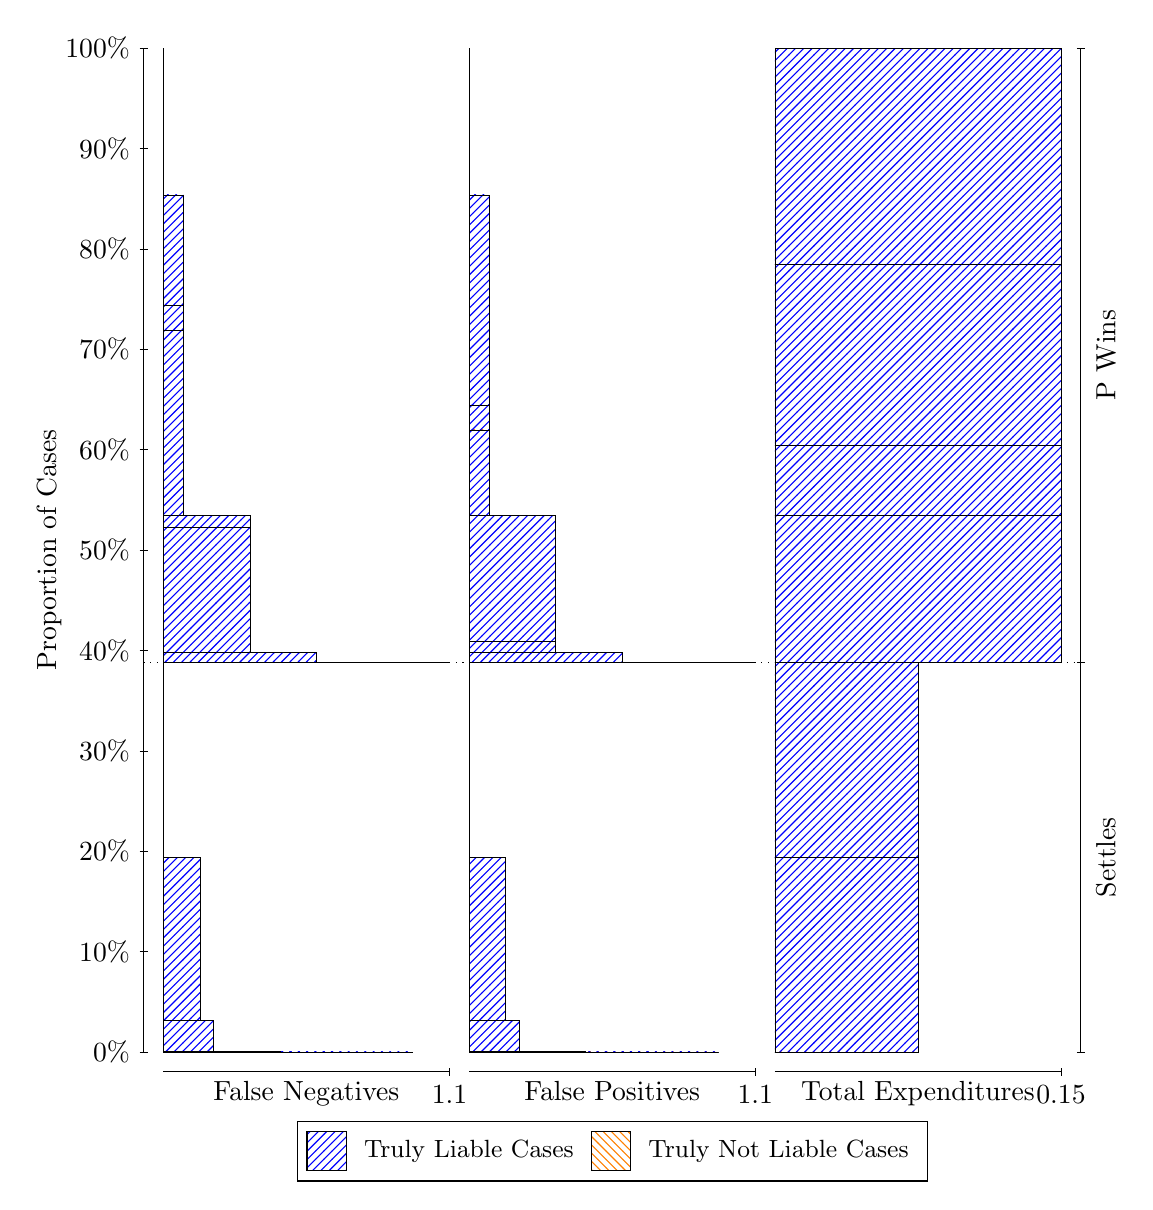
\begin{tikzpicture}
\draw[black, very thin] (1.5,1.75) -- (1.5,14.5);
\node[rotate=90, anchor=center] at (0.3, 8.125) {Proportion of Cases};
\draw[black, very thin] (1.45,1.75) -- (1.55,1.75);
\node[anchor=east] at (1.45, 1.75) {0\%};
\draw[black, very thin] (1.45,3.025) -- (1.55,3.025);
\node[anchor=east] at (1.45, 3.025) {10\%};
\draw[black, very thin] (1.45,4.3) -- (1.55,4.3);
\node[anchor=east] at (1.45, 4.3) {20\%};
\draw[black, very thin] (1.45,5.575) -- (1.55,5.575);
\node[anchor=east] at (1.45, 5.575) {30\%};
\draw[black, very thin] (1.45,6.85) -- (1.55,6.85);
\node[anchor=east] at (1.45, 6.85) {40\%};
\draw[black, very thin] (1.45,8.125) -- (1.55,8.125);
\node[anchor=east] at (1.45, 8.125) {50\%};
\draw[black, very thin] (1.45,9.4) -- (1.55,9.4);
\node[anchor=east] at (1.45, 9.4) {60\%};
\draw[black, very thin] (1.45,10.675) -- (1.55,10.675);
\node[anchor=east] at (1.45, 10.675) {70\%};
\draw[black, very thin] (1.45,11.95) -- (1.55,11.95);
\node[anchor=east] at (1.45, 11.95) {80\%};
\draw[black, very thin] (1.45,13.225) -- (1.55,13.225);
\node[anchor=east] at (1.45, 13.225) {90\%};
\draw[black, very thin] (1.45,14.5) -- (1.55,14.5);
\node[anchor=east] at (1.45, 14.5) {100\%};

\draw[black, very thin] (13.4,1.75) -- (13.4,14.5);
\draw[black, very thin] (13.35,1.75) -- (13.45,1.75);
\node[anchor=west] at (13.35, 1.75) {};
\draw[black, very thin] (13.35,6.6985) -- (13.45,6.6985);
\node[anchor=west] at (13.35, 6.6985) {};
\draw[black, very thin] (13.35,14.5) -- (13.45,14.5);
\node[anchor=west] at (13.35, 14.5) {};

\draw[black, very thin, pattern color=blue, pattern=north east lines] (1.75,1.75) rectangle (4.9186,1.75);
\draw[black, very thin, pattern color=blue, pattern=north east lines] (1.75,1.75) rectangle (4.0736,1.75);
\draw[black, very thin, pattern color=blue, pattern=north east lines] (1.75,1.75) rectangle (3.5667,1.75);
\draw[black, very thin, pattern color=blue, pattern=north east lines] (1.75,1.75) rectangle (3.2287,1.7534);
\draw[black, very thin, pattern color=blue, pattern=north east lines] (1.75,1.7534) rectangle (2.7217,1.7534);
\draw[black, very thin, pattern color=blue, pattern=north east lines] (1.75,1.7534) rectangle (2.3837,2.1551);
\draw[black, very thin, pattern color=blue, pattern=north east lines] (1.75,2.1551) rectangle (2.2147,4.2242);
\draw[black, very thin, pattern color=blue, pattern=north east lines] (1.75,4.2242) rectangle (1.8767,4.2242);
\draw[black, very thin, pattern color=orange, pattern=north west lines] (1.75,4.2242) rectangle (1.75,4.2242);
\draw[black, very thin, pattern color=blue, pattern=north east lines] (1.75,4.2242) rectangle (1.75,6.6985);
\draw[black, very thin, pattern color=blue, pattern=north east lines] (1.75,6.6985) rectangle (5.3833,6.6985);
\draw[black, very thin, pattern color=blue, pattern=north east lines] (1.75,6.6985) rectangle (4.5384,6.6997);
\draw[black, very thin, pattern color=blue, pattern=north east lines] (1.75,6.6997) rectangle (3.6934,6.8199);
\draw[black, very thin, pattern color=blue, pattern=north east lines] (1.75,6.8199) rectangle (2.8484,8.4148);
\draw[black, very thin, pattern color=blue, pattern=north east lines] (1.75,8.4148) rectangle (2.8484,8.5626);
\draw[black, very thin, pattern color=blue, pattern=north east lines] (1.75,8.5626) rectangle (2.0035,10.911);
\draw[black, very thin, pattern color=blue, pattern=north east lines] (1.75,10.911) rectangle (2.0035,11.229);
\draw[black, very thin, pattern color=blue, pattern=north east lines] (1.75,11.229) rectangle (2.0035,12.636);
\draw[black, very thin, pattern color=orange, pattern=north west lines] (1.75,12.636) rectangle (1.75,12.636);
\draw[black, very thin, pattern color=blue, pattern=north east lines] (1.75,12.636) rectangle (1.75,14.5);
\draw[black, very thin, pattern color=orange, pattern=north west lines] (5.6333,1.75) rectangle (8.8019,1.75);
\draw[black, very thin, pattern color=blue, pattern=north east lines] (5.6333,1.75) rectangle (8.8019,1.75);
\draw[black, very thin, pattern color=blue, pattern=north east lines] (5.6333,1.75) rectangle (7.957,1.75);
\draw[black, very thin, pattern color=orange, pattern=north west lines] (5.6333,1.75) rectangle (7.45,1.75);
\draw[black, very thin, pattern color=blue, pattern=north east lines] (5.6333,1.75) rectangle (7.45,1.75);
\draw[black, very thin, pattern color=blue, pattern=north east lines] (5.6333,1.75) rectangle (7.112,1.7534);
\draw[black, very thin, pattern color=blue, pattern=north east lines] (5.6333,1.7534) rectangle (6.605,1.7534);
\draw[black, very thin, pattern color=blue, pattern=north east lines] (5.6333,1.7534) rectangle (6.2671,2.1551);
\draw[black, very thin, pattern color=orange, pattern=north west lines] (5.6333,2.1551) rectangle (6.0981,2.1551);
\draw[black, very thin, pattern color=blue, pattern=north east lines] (5.6333,2.1551) rectangle (6.0981,4.2243);
\draw[black, very thin, pattern color=blue, pattern=north east lines] (5.6333,4.2243) rectangle (5.7601,4.2243);
\draw[black, very thin, pattern color=blue, pattern=north east lines] (5.6333,4.2243) rectangle (5.6333,6.6985);
\draw[black, very thin, pattern color=orange, pattern=north west lines] (5.6333,6.6985) rectangle (9.2667,6.6985);
\draw[black, very thin, pattern color=blue, pattern=north east lines] (5.6333,6.6985) rectangle (9.2667,6.6985);
\draw[black, very thin, pattern color=orange, pattern=north west lines] (5.6333,6.6985) rectangle (8.4217,6.6985);
\draw[black, very thin, pattern color=blue, pattern=north east lines] (5.6333,6.6985) rectangle (8.4217,6.6997);
\draw[black, very thin, pattern color=orange, pattern=north west lines] (5.6333,6.6997) rectangle (7.5767,6.6997);
\draw[black, very thin, pattern color=blue, pattern=north east lines] (5.6333,6.6997) rectangle (7.5767,6.8199);
\draw[black, very thin, pattern color=orange, pattern=north west lines] (5.6333,6.8199) rectangle (6.7318,6.8199);
\draw[black, very thin, pattern color=blue, pattern=north east lines] (5.6333,6.8199) rectangle (6.7318,6.9677);
\draw[black, very thin, pattern color=blue, pattern=north east lines] (5.6333,6.9677) rectangle (6.7318,8.5626);
\draw[black, very thin, pattern color=blue, pattern=north east lines] (5.6333,8.5626) rectangle (5.8868,9.6508);
\draw[black, very thin, pattern color=orange, pattern=north west lines] (5.6333,9.6508) rectangle (5.8868,9.6508);
\draw[black, very thin, pattern color=blue, pattern=north east lines] (5.6333,9.6508) rectangle (5.8868,9.9693);
\draw[black, very thin, pattern color=blue, pattern=north east lines] (5.6333,9.9693) rectangle (5.8868,12.636);
\draw[black, very thin, pattern color=blue, pattern=north east lines] (5.6333,12.636) rectangle (5.6333,14.5);
\draw[black, very thin, pattern color=orange, pattern=north west lines] (9.5167,1.75) rectangle (11.333,1.75);
\draw[black, very thin, pattern color=blue, pattern=north east lines] (9.5167,1.75) rectangle (11.333,4.2242);
\draw[black, very thin, pattern color=orange, pattern=north west lines] (9.5167,4.2242) rectangle (11.333,4.2242);
\draw[black, very thin, pattern color=blue, pattern=north east lines] (9.5167,4.2242) rectangle (11.333,6.6985);
\draw[black, very thin, pattern color=orange, pattern=north west lines] (9.5167,6.6985) rectangle (13.15,6.6985);
\draw[black, very thin, pattern color=blue, pattern=north east lines] (9.5167,6.6985) rectangle (13.15,8.5686);
\draw[black, very thin, pattern color=orange, pattern=north west lines] (9.5167,8.5686) rectangle (13.15,8.5686);
\draw[black, very thin, pattern color=blue, pattern=north east lines] (9.5167,8.5686) rectangle (13.15,9.4499);
\draw[black, very thin, pattern color=orange, pattern=north west lines] (9.5167,9.4499) rectangle (13.15,9.4499);
\draw[black, very thin, pattern color=blue, pattern=north east lines] (9.5167,9.4499) rectangle (13.15,11.749);
\draw[black, very thin, pattern color=orange, pattern=north west lines] (9.5167,11.749) rectangle (13.15,11.749);
\draw[black, very thin, pattern color=blue, pattern=north east lines] (9.5167,11.749) rectangle (13.15,14.5);
\draw[black, dotted] (1.5,6.6985) -- (13.4,6.6985);
\draw[black, very thin] (1.75,1.5) -- (5.3833,1.5);
\node[anchor=north] at (3.5667, 1.5) {False Negatives};
\draw[black, very thin] (5.3833,1.45) -- (5.3833,1.55);
\node[anchor=north] at (5.3833, 1.45) {1.1};

\draw[black, very thin] (5.6333,1.5) -- (9.2667,1.5);
\node[anchor=north] at (7.45, 1.5) {False Positives};
\draw[black, very thin] (9.2667,1.45) -- (9.2667,1.55);
\node[anchor=north] at (9.2667, 1.45) {1.1};

\draw[black, very thin] (9.5167,1.5) -- (13.15,1.5);
\node[anchor=north] at (11.333, 1.5) {Total Expenditures};
\draw[black, very thin] (13.15,1.45) -- (13.15,1.55);
\node[anchor=north] at (13.15, 1.45) {0.15};

\node[black, centered, rotate=90] at (13.72, 4.2242) {Settles};
\node[black, centered, rotate=90] at (13.72, 10.599) {P Wins};

\draw (7.449999999999999,1.5) node[draw=none] (baseCoordinate) {};
\begin{scope}[align=center]
        \matrix[scale=0.5, draw=black, below=0.5cm of baseCoordinate, nodes={draw}, column sep=0.1cm]{
            \node[rectangle, draw, minimum width=0.5cm, minimum height=0.5cm, pattern=north east lines, pattern color=blue] {}; &
            \node[draw=none, font=\small] (B) {Truly Liable Cases}; &
            \node[rectangle, draw, minimum width=0.5cm, minimum height=0.5cm, pattern=north west lines, pattern color=orange] {}; &
            \node[draw=none, font=\small] (B) {Truly Not Liable Cases}; \\
            };
\end{scope}

\end{tikzpicture}
\end{document}